\documentclass{article}
\usepackage{graphicx}
\usepackage{float}
\usepackage{amsmath}
\usepackage{amsfonts}
\usepackage{amssymb}
\usepackage{hyperref}
\usepackage{esint}
\usepackage[utf8]{inputenc}
\usepackage[a4paper, portrait, margin=0.75in]{geometry}
\setlength\parindent{0pt}
\usepackage[italian]{babel}



\hypersetup{
    colorlinks=true,
    linkcolor=black,
    filecolor=magenta,
    urlcolor=blue,
    pdftitle={Tecnologie internet},
    pdfpagemode=FullScreen,
}


\begin{document}
    \author{Dmitri Ollari Ischimji\\dmotrio.xyz}
    \title{Ingegneria dei software}

    \maketitle
    \tableofcontents

    \listoffigures
    \listoftables

    \newpage

\section{T1 - Software Development Process}
L'Ingegneria del Software non è solo scrivere codice è piuttosto un concetto 
di risoluzione dei problemi del mondo reale sfruttando il software.

I requisiti sono sempre più stringenti: tempi brevi, sistemi complessi, molte features.

Un buon software deve avere ottime \textbf{maintenability, dependability, efficiency, acceptability}.

I problemi e le soluzioni sono sempre complesse ma il software permette massima flessibilità.
È un sistema discreto.

Le sfide principali sono rappresentate da \textbf{eterogeneità, delivery, trust}.

La fase di problem solving si suddivide in analisi e sitesi.

\subsection{Cos'è l'ingegneria del software?}
L'Ingegneria del software è un \textbf{insieme di tecniche, metodologie, strumenti} che aiutano
nella produzione di software di alta qualità dati un budget, una scadenza, e delle modifiche continue.

La sfida principale è quelli di aver a che fare con complessità elevate e ad un aumento delle
responsabilità, dato che un ingegnere del software non deve solo scrivere codice, ma piuttosto lavorare
con competenza e confidenzialità, attenendosi ad un'etica.

\subsubsection{Processo del software}
Dopo una rappresentazione astratta, si procede con un set di attività strutturate:
specifiche dei \textbf{requirements, design, implementazione, validazione, evoluzione.}

\subsection{Modelli di sviluppo del software}
Distinguiamo tra \textbf{plan-driven} e \textbf{agile} development. Nel primo si pianificano 
i requisiti e solo in seguito si sviluppa il software. Nel secondo si sviluppa il software un pezzo alla
volta, a stretto contatto con il cliente per dei feedback.

\subsubsection{Modello a cascata}
Modello plan-driven, le specifiche e lo sviluppo sono separati.

I pro:
\begin{itemize}
    \item ottima documentazione
    \item manutenzione semplice
\end{itemize}

I cons:
\begin{itemize}
    \item specifiche congelate dopo la pianificazione iniziale
    \item cliente poco coninvolto
    \item tempi lunghi
\end{itemize}

\begin{figure}[h!]
    \centering
    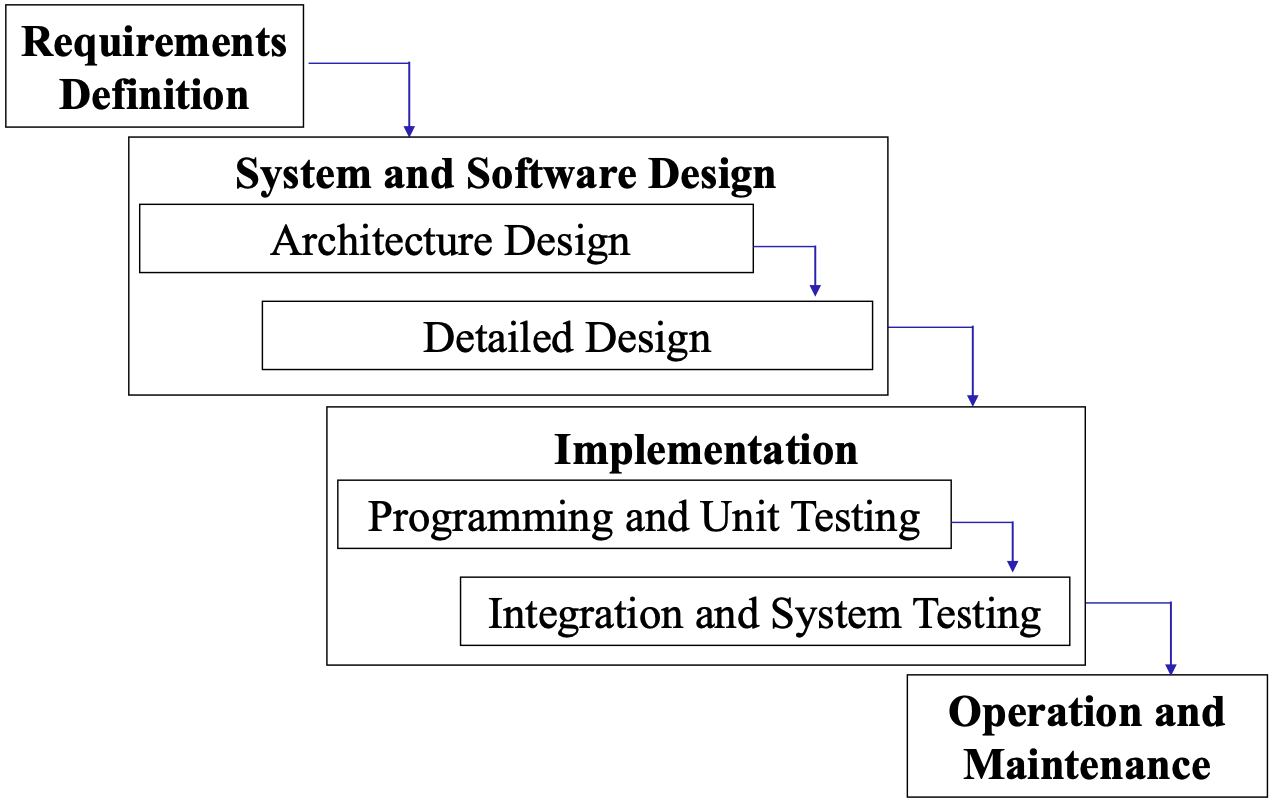
\includegraphics[width=0.5\linewidth]{imgs/1 - cascata.png}
    \label{fig:modello_cascata}
    \caption{Modello a cascata}
\end{figure}

\subsubsection{Modello a spirale}
Diverse fasi che susseguono a spirale, la gestione del rischio viene gestita
tramite prototipazione che permette di testare i prodotti.

I pro:
\begin{itemize}
    \item prevenzione dei rischi
    \item completezza della documentazione
    \item flessibilità
    \item elevata usabilità
    \item buon design
    \item facilità di manutenzione
    \item ridotto costo di sviluppo
\end{itemize}

I cons:
\begin{itemize}
    \item modello costoso
    \item riservato ad esperti e a progetti costosi
\end{itemize}

Il prototipo è un'implementazione limitata del sistema, rappresentanti solo alcuni aspetti alla volta.

\begin{figure}[h!]
    \centering
    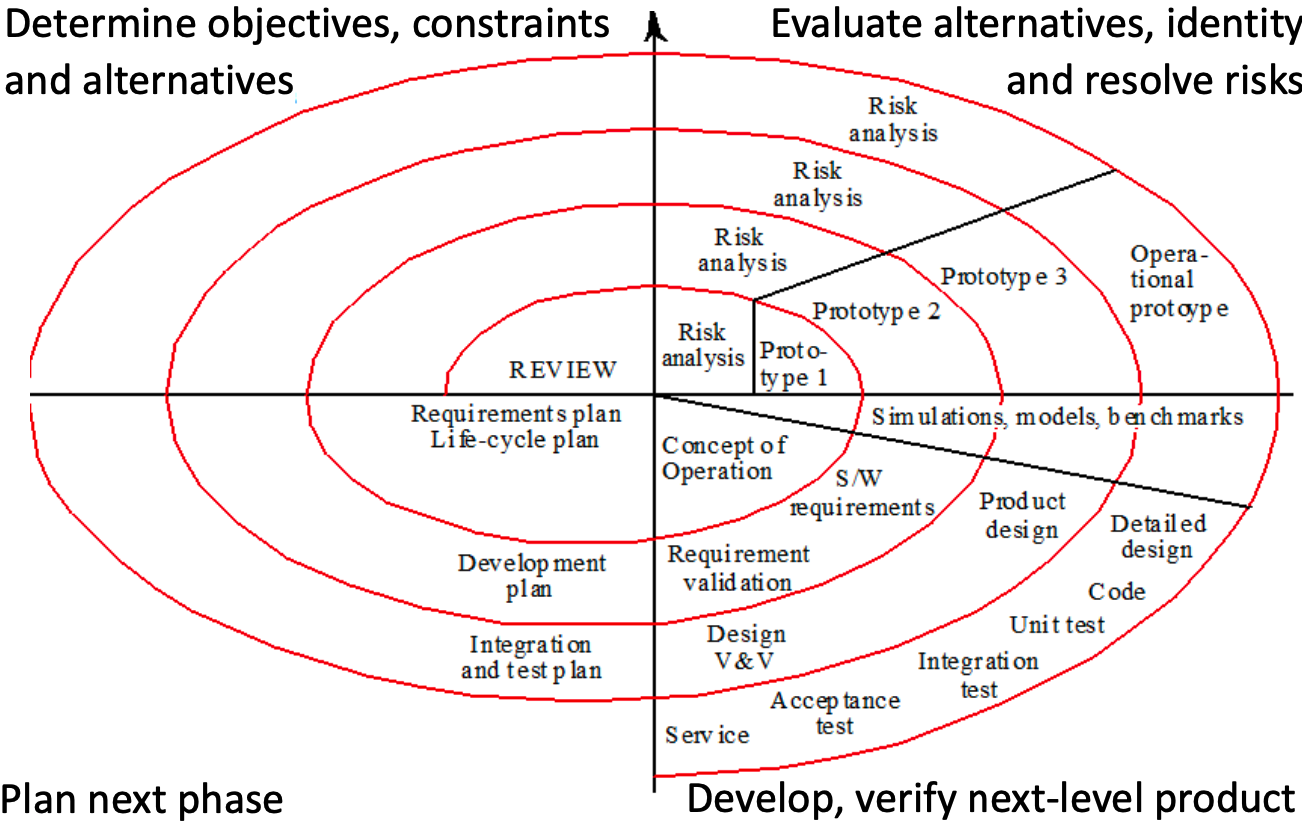
\includegraphics[width=0.5\linewidth]{imgs/2 - spirale.png}
    \label{fig:modello_spirale}
    \caption{Modello a spirale}
\end{figure}

\subsubsection{Sviluppo incrementale}
Modello che si suddivide in fasi:
\begin{enumerate}
    \item raccolta dei requisiti
    \item versione iniziale
    \item fase di design
    \item fase di implementazione
    \item produzione di versione finale
\end{enumerate}

I pro:
\begin{itemize}
    \item naturale presenza di prototipi ad ogni aggiunta di features
    \item basso rischio di fallimento
    \item qualità di testing in base alla priorità
\end{itemize}

I cons:
\begin{itemize}
    \item scarsa visibilità d'insieme
    \item sistemi mal strutturati
    \item skill speciali necessarie
\end{itemize}

Adatto a progetti piccoli o parti di progetti grandi.

\begin{figure}[h!]
    \centering
    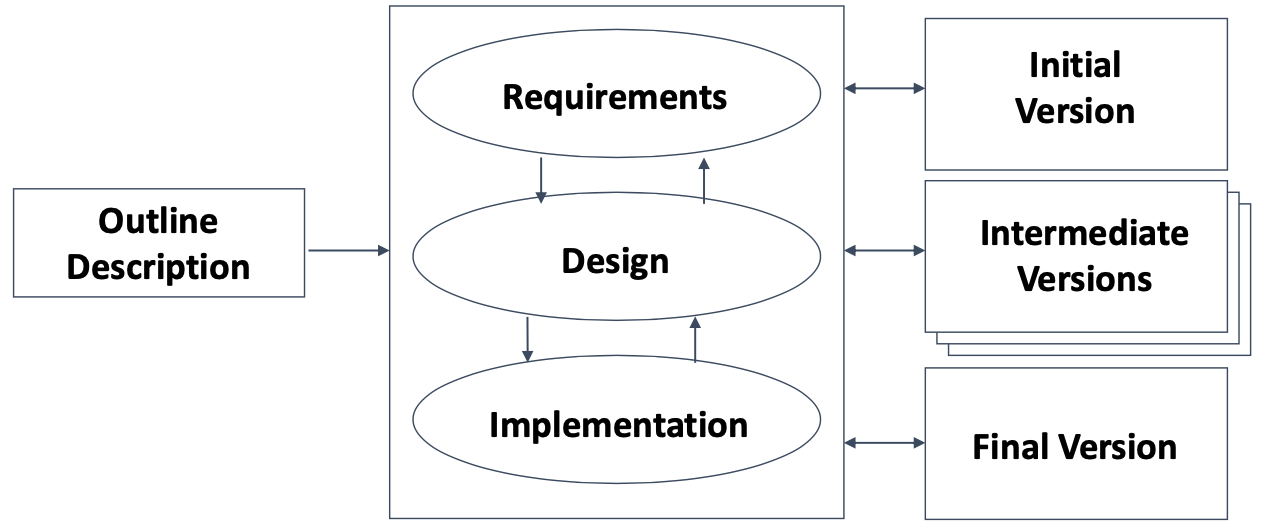
\includegraphics[width=0.5\linewidth]{imgs/3 - incrementale.png}
    \label{fig:modello_incrementale}
    \caption{Modello a incrementale}
\end{figure}

\subsubsection{Sviluppo guidato dai test}
Vengono prima scritti i test e poi l'implementazione mettendo le difficolta in primo piano.

Rende il debug più semplice.

Si aggiunte il nuovo test e poi la features cosi da veriicare che tutti i test 
precedenti siano validi.

\subsubsection{Sviluppo agile}
Questo modello di sviluppo è basato sul concetto di delivery del prodotto continuo 
avendo delle features in continua evoluzione.

Il cliente è al centro dello sviluppo, il team si autoorganizza e le features 
vengono aggiunte man mano.

Essendoci la mancanza di planning il team deve essere esperto per non perdersi.


Spesso si creano documentazioni sbagliate o incomplete.

\subsubsection{Extrem programming}
L' XP viene scelte quado i requisiti cambiano velocemente, i team sono ridotti
e affiatati(pair programming per esempio).

Tipo di programmazione agile, basato sul design semplice, release minori,
refactoring continuo, alta semplicità.

\begin{figure}[h!]
    \centering
    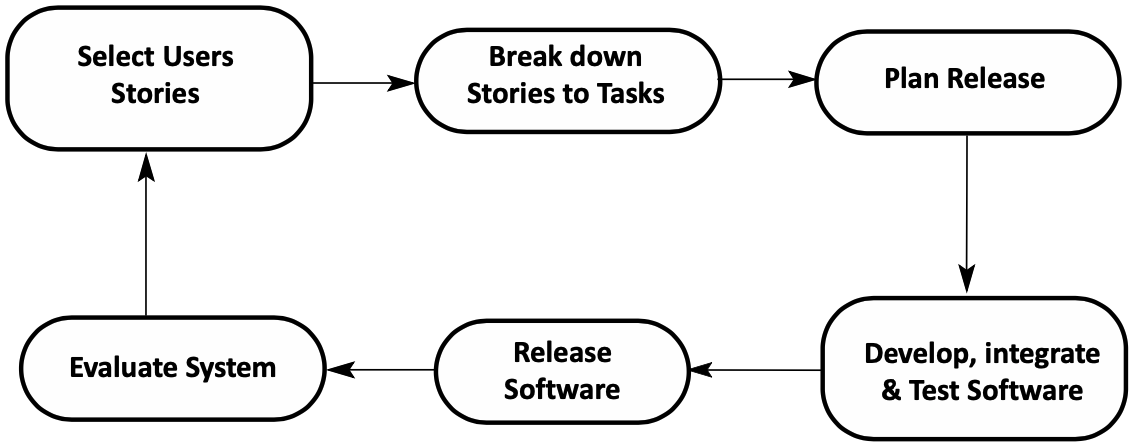
\includegraphics[width=0.5\linewidth]{imgs/4 - xp.png}
    \label{fig:modello_xp}
    \caption{Modello a extrem programming}
\end{figure}

\subsection{Software riusabile}

È comodo lavorare per \textbf{microservizi atomici}, di modo da usarli in seguito 
se si affronta un problema simile, un'esempio sono le API, è sempre meglio riusare qualcosa 
che riscriverlo da zero.

Questo "\textit{mindset}" riduce i temi e i costi di sviluppo nel luno periodo.

Il contro è il fatto che i microservizi non sono fatti espressamente per una task specifica
e si va a sacrificare qualche requisito.


\section{T2 - Coding, Debugging, Testing}
Lo stile di coding è importante perchè un programma viene scritto una volta e letto
spesso da altri!

Stare a ttenti ai layout, nomi, commenti, ecc\dots

\subsection{Legge di Ambler per gli standard}
Più uno standard è adottato e più sarà facile farlo usare al proprio team.

Non perdere tempo adietro a standard scemi.

Se hai dei dubbi usa gli standaard di google che sicuramente ne sanno più di me e te.
\textbf{\href{https://google.github.io/styleguide/}{standard di google}}


Solitamente si hanno degli standard aziendali e questi standard vanno a chiarire aspetti come:
\begin{itemize}
    \item nomenclatura
    \item formattazione
    \item formato
    \item contenuto
\end{itemize}

\subsection{Coding practices}
\begin{itemize}
    \item indentazione
    \item whitespaces
    \item naming, commenting
\end{itemize}

Fondaentale è spiegare i compiti delle classi, funzioni e procecssi complessi.

Utilizzare uno standard permette ai collechi di non dover riscrivere il codice.
Rendendo più semplice le iterazioni del codice successive.

\subsection{Gestione degli errori}
Si fa un distinguo fra il prima, durante e dopo:
\begin{itemize}
    \item prrevenzione
    \item rilevamento
    \item recupero
\end{itemize}

Per debuggare, bisogna riconoscere l'errore, isolare la fonte, identificarne la causa,
trovare un fix, applicarlo e testarlo.

\subsection{Testing}
Permette di trovare errori ma non la loro assenza, \textbf{il tester non dovrebbe
essere il programmatore}.

\subsubsection{Unit testing}
Test di singoli componenti.

\subsubsection{Integration testing}

L'intero sistema è visto come insieme di sottositemi, l'obbiettivo è quello di testare tutte le interfacce e le 
interazioni fra i sottositemi.

\subsubsection{System testing}
test dell'intero sistema per vedere se rispetta i requisiti funzionali.

\subsubsection{Functional testing}

Verifica delle funzionalità del sistema, test basati sui requisiti del progetto.

\subsubsection{Performance testing}
Test in situazioni estreme(stress testing, volume testing, recovery testing, penetration testing).

\subsubsection{Acceptance testing}
Il sistema è pronto per la produzione??

Test scelti ed effettuati dal cliente.(alpha e beta test)

\section{T3 - System Modelling and UML}

Rappresentazione astratta del sistema e dei problemi, si dedvono introdurre i componenti essenziali mediante una noazione
consistente.

Il system modelling deve essere \textbf{predictive}(prima del development), \textbf{extracted}(da un sistema 
esistente) e \textbf{prescriptive}(definire regole per l'evoluzione del software).

\subsection{UML}
UML è semplice, espressivo, utile, consistent, estensibile.

\section{T4 - Requirements engineering}




























































\end{document}

